\chapter{Performance-Analyse der derzeitigen Implementierung}

\section{Komplexität}

\subsection{Speckle-Tracking}

Der erste Schritt des Speckle-Trackings ist die Feststellung der starren Verschiebung. Werden hierfür feste Werte angenommen, ist diese Komplexität konstant. Wird allerdings ein Korrelationsverfahren verwendet, so ist die Komplexität $\mathcal{O}(\gls{resolution} \cdot log(\gls{resolution}))$ für die \glsfirst{resolution} \glssymbol{resolution}, da hierfür \glspl{FFT} eingesetzt werden. 

Der nächste Verarbeitungsschritt ist der erste Durchlauf. Hier werden die Eingabebilder zunächst durch die Selektion der \gls{ROI}, also auf die \glsfirst{rroi} \glssymbol{rroi} verkleinert und anschließend in Blöcke mit konstanter Größe aufgeteilt, welche dann ineinander mittels des Template-Matchings gesucht werden. Die Komplexität der einzelnen Suchvorgänge kann somit auch als konstant angesehen werden. Der Durchlauf braucht demzufolge $\mathcal{O}(\gls{rroi})$ Schritte. Die anschließende Interpolation wird auf alle Pixel des Bildes angewandt und hat demzufolge eine Komplexität von $\mathcal{O}(\gls{rroi})$.

Der zweite Durchlauf, der als nächstes folgt, werden Subbilder, wie \ref{sec:speckle-tracking} beschrieben, generiert. durch die \glsfirst{uap} \glssymbol{uap} wird \gls{rroi}, und damit auch die Komplexität dieses Teils, mit dem Faktor $\gls{uap}^2$ verringert. Die \glsfirst{corrsize} \glssymbol{corrsize} legt nimmt auf das Template-Matching Einfluss, dessen Komplexität nun bei $\mathcal{O}(\gls{corrsize} \cdot log(\gls{corrsize}))$ liegt. Der Einfluss der \glsfirst{gridResol} \glssymbol{gridResol} ist, ähnlich zu \gls{uap}, eine Verringerung mit dem Faktor $\gls{gridResol}^2$. Die Gesamtkomplexität der Template-Matchings im zweiten Durchlauf liegt somit bei:

\begin{center}
	$\mathcal{O}(\frac{\gls{rroi} \cdot \gls{corrsize} \cdot log(\gls{corrsize})}{(\gls{uap}^2 \cdot \gls{gridResol})^2})$
\end{center}

Für die auf den Template-Matching-Prozess folgende Subpixel-Interpolierung werden neun Pixel in der Umgebung des Maximums jedes Übereinstimmungsmatrix interpoliert, womit dieser Schritt folgende Komplexität aufweist:

\begin{center}
	$\mathcal{O}(\frac{\gls{rroi}}{(\gls{uap}^2 \cdot \gls{gridResol}^2)})$
\end{center}

Am Ende des Speckle-Tracking-Algorithmus wird versucht, nicht zuordenbare Ergebnisse mit einer anderen \glsfirst{corrsize} \glssymbol{corrsize} erneut zuzuordnen. Im schlimmsten Fall wird der zweite Durchlauf für die Hälfte der Subbilder \gls{ncorr}-fach wiederholt, wobei \gls{ncorr} die \glsdesc{ncorr} repräsentiert. Bei höheren Fehlerraten über 50\% bricht das Programm. In der hier als Grundlage vorliegenden Implementierung ist $\gls{ncorr} = 6$.

Die Gesamtkomplexität des Speckle-Tracking-Algorithmus liegt damit in der Komplexitätsklasse:

\begin{center}
	$\mathcal{O}(\frac{\gls{rroi} \cdot \gls{corrsize} \cdot log(\gls{corrsize})}{(\gls{uap}^2 \cdot \gls{gridResol})^2})$
\end{center}

\subsection{Gradientenintegration}

Um eine effiziente Integration der Gradienten zu ermöglichen, beruht der von \citeauthor{FC88} vorgeschlagene Algorithmus auf der Integration im Frequenzraum. Hierzu werden zuerst die Gradientenbilder mittels \glspl{FFT} in diesen Raum transformiert, dort in linearer Komplexität integriert und zum Schluss wieder zurück transformiert. 
Aufgrund der Verwendung von \glspl{FFT} befindet sich dieser Algorithmus in der Komplexitätsklasse:

\begin{center}
	$\mathcal{O}(\gls{resolution} \cdot log(\gls{resolution}))$
\end{center}

\subsection{Kalibrierung}

Die Komplexität der Parameterinitialisierung innerhalb der Kalibrierungsroutine ist trivial und kann daher als linear angenommen werden. 

Während der Dunkelfeldkalibrierung wird ein Medianbild aus \gls{N} Bildern erstellt. Für diese \gls{N} Bilder wird an jeder Position des Bildes der Median gebildet. Somit ist dieser Teil des Algorithmus in der Komplexitätsklasse:

\begin{center}
	$\mathcal{O}(\gls{N} \cdot \gls{resolution})$
\end{center}

Die Nullfeldkalibrierung verläuft sehr ähnlich. Hier wird ein Durchschnittsbild aus \gls{N} Bildern erstellt, für welches alle Pixel  der \gls{N} Bilder an der selben Position aufaddiert und anschließend durch \gls{N} geteilt werden. Somit ist auch dieser Teil des Algorithmus in der Komplexitätsklasse:

\begin{center}
	$\mathcal{O}(\gls{N} \cdot \gls{resolution})$
\end{center}

Nachdem diese Kalibrierungen abgeschlossen sind, folgt die Hauptschleife in der die Sensorstreuung mittels des Speckle-Tracking-Algorithmus aus allen möglichen Bildpaarkombinationen $\gls{N}^2$ berechnet wird. Hierzu werden zuerst die Sensorbilder mittels der bei der Kalibrierung ermittelten Werte mit einer Komplexität von $\mathcal{O}(\gls{resolution})$ korrigiert und anschließend bestimmt der Speckle-Tracking-Algorithmus die Streuung des Sensors. Die gesamte Streueffeckterkennung hat somit eine Komplexität von: 

\begin{center}
	$\mathcal{O}(\frac{\gls{N}^2 \cdot\gls{rroi} \cdot \gls{corrsize} \cdot log(\gls{corrsize})}{(\gls{uap}^2 \cdot \gls{gridResol})^2})$
\end{center}

Dies liegt insbesondere für kleine \gls{uap} und \gls{gridResol} in der Komplexitätsklasse:

\begin{center}
	$\mathcal{O}(\gls{N}^2 \cdot\gls{rroi} \cdot \gls{corrsize} \cdot log(\gls{corrsize}))$
\end{center}

Da die Streueffekterkennung deutlich komplexer als der Rest der Kalibrierungsphase ist, liegt die Komplexität dieser ebenfalls in der oben beschriebenen Komplexitätsklasse. 

\subsection{Hauptroutine}

Ähnlich zur Kalibrierung beginnt die Hauptroutine mit einer linearen Parameterinitialisierung. Auf diese folgt die Hauptschleife, welche für die \gls{N_Paare} jeweils ein mal ausgeführt wird. Genau, wie in der Kalibrierung wird auch hier wieder eine Korrektor der Eingabebilder in linearer Zeit vorgenommen. Dies wird gefolgt vom Speckle-Tracking-Algorithmus und der Gradientenintegration. Die höchste Komplexität hat hier auch wieder der Template-Matching-Algorithmus, welcher damit die Komplexitätsklasse und somit auch der gesamten Hauptroutine festlegt auf:

\begin{center}
	$\mathcal{O}(\frac{\gls{N_Paare} \cdot\gls{rroi} \cdot \gls{corrsize} \cdot log(\gls{corrsize})}{(\gls{uap}^2 \cdot \gls{gridResol})^2})$
\end{center}

Dies liegt, ähnlich zur Kalibrierung, für kleine \gls{uap} und \gls{gridResol} in der Komplexitätsklasse:

\begin{center}
	$\mathcal{O}(\gls{N_Paare} \cdot\gls{rroi} \cdot \gls{corrsize} \cdot log(\gls{corrsize}))$
\end{center}

\section{Benchmark}

\subsection{Testsystem und Laufzeitumstände}

\paragraph{Testsystem}

Alle Benchmarks liefen auf den \textit{haswell}-Partition des Taurus-Supercomputers an der Technischen Universität Dresden. Jeder Knote dieser Partition ist ausgestattet mit zwei Intel\textregistered Xeon\textregistered E5-2680 v3 \glspl{CPU}. Diese haben zwölf Rechenkerne, die mit bis zu 2.50 GHz getaktet sind. MultiThreading war hierbei nicht aktiviert. Die Knoten haben 64 GiB (\textit{haswell64}), 128 GiB (\textit{haswell128}) oder 256 GiB (\textit{haswell256}) Arbeitsspeicher zur Verfügung. Zusätzlich ist pro Rechenknoten eine 128 GB \gls{SSD} installiert. Es wurde unter anderem Python 2.7.11 mit numpy 1.10.1 und OpenCV 3.1.0 verwendet. Eine komplette Liste aller geladenen Module lässt sich \correctme{hier} finden.

\paragraph{Laufzeitumstände}

Jede Konfiguration, bestehend aus Datensatz und Kernanzahl, wurde nach vier Aufwärmiterationen fünf mal ausgeführt. Hierbei wurden jeweils die reinen Ausführungszeiten des gesamten Skripts und einzelner Funktionen erfasst. Aus allen vorliegenden Zeiten wurde \gls{IO}-Zeiten herausgerechnet. Die Laufzeit mit den entsprechenden Datensätzen wurde auf unterschiedlich vielen Kernen von eins bis 24 gemessen. Jeder Benchmark lief exklusiv auf einem Knoten.  \correctme{-> Referenz zu Tabelle}

\paragraph{Datensätze}

Zur Leistungsfeststellung der vorliegenden Implementierung werden drei verschiedene Arten von Datensätzen verwendet: \textit{detectorDistortion}, \textit{Experiment 6}, \textit{Lenses}. \textit{detectorDistortion} wird zur Kalibrierung verwendet. Die Eigenschaften dieser Typen werden in Tabelle \ref{tab:datasets} gegenüber gestellt.  Von diesem Datensatztyp gibt es einen Datensatz mit 25 Bildern. Es existieren drei \textit{Experiment 6} Datensätze mit 21 (\textit{Experiment 6 Lenses 200}), 11 (\textit{Experiment 6 Lenses 500}) und 14 Bildpaaren (\textit{Experiment 6 Lenses 1500}). Vom letzten Typ existieren vier Datensätze mit jeweils zehn (\textit{Lenses Set 1}), fünf (\textit{Lenses Set 2}), zwei (\textit{Lenses Set 3}) und einem Bildpaar.

\begin{table}
	\begin{tabularx}{\textwidth}{| X || X || X | X |}
		\hline
		& \textbf{Kalibrierung} & \multicolumn{2}{c|}{\textbf{Hauptroutine}} \\
		\cline{2-4}
		& detectorDistortion & Experiment 6 & Lenses \\
		\hline
		\hline
		\gls{rroi} (in Pixel) & 1848 x 1848 & Sensor 1: 1450 x 1450 \newline
		Sensor 2: 550 x 550 & 1450 x 1550 \\
		\hline
		\gls{gridResol} & 4 & 1 & 1 \\
		\hline
		\gls{corrsize} & 37 & 91 & 41 \\
		\hline
		\gls{uap} & 1 & 1 & 1 \\
		\hline
		Pixelgröße & gleich & unterschiedlich & gleich \\
		\hline
	\end{tabularx}
	\caption{Parameter der Datensätze}
	\label{tab:datasets}
\end{table}

\subsection{Laufzeiten}

\begin{correctmore}
	TODO
\end{correctmore}

\begin{center}
\begin{figure}[htbp]
	\begin{subfigure}[b]{0.325\textwidth}
		\centering
		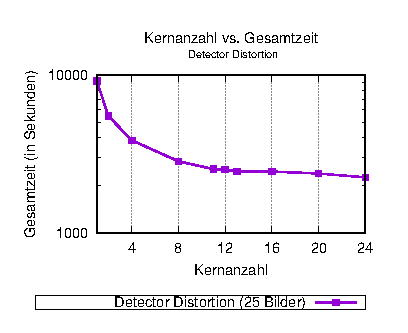
\includegraphics[width=\textwidth]{pdf/times_detector_distortion}
		\caption[Detector Distortion]{Detector Distortion}
		\label{fig:times_det_dist}
	\end{subfigure}
	\hfill
	\begin{subfigure}[b]{0.325\textwidth}
		\centering
		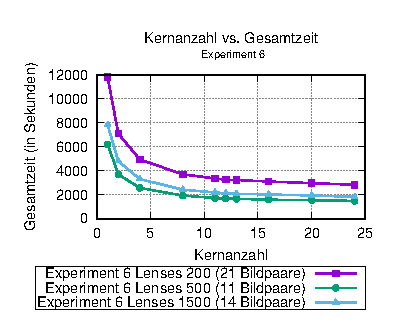
\includegraphics[width=\textwidth]{pdf/times_exp6}
		\caption[Experiment 6]{Experiment 6}
		\label{fig:times_exp6}
	\end{subfigure}
	\hfill
	\begin{subfigure}[b]{0.325\textwidth}
		\centering
		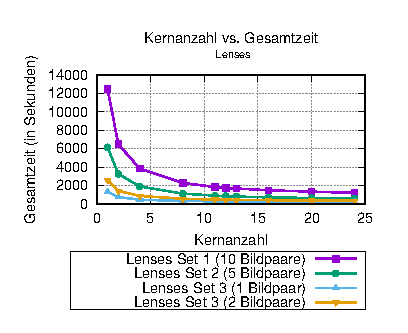
\includegraphics[width=\textwidth]{pdf/times_lenses}
		\caption[Lenses]{Lenses}
		\label{fig:times_lenses}
	\end{subfigure}
	\caption{Gesamtlaufzeiten}
\end{figure}
\end{center}

\begin{center}
\begin{figure}[htbp]
	\begin{subfigure}[b]{0.325\textwidth}
		\centering
		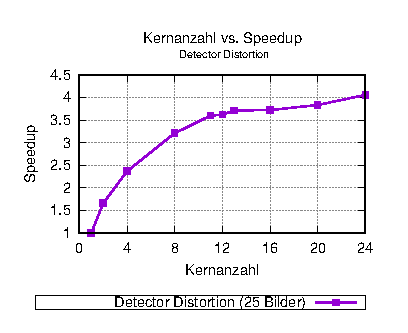
\includegraphics[width=\textwidth]{pdf/speedup_detector_distortion}
		\caption[Detector Distortion]{Detector Distortion}
		\label{fig:speedup_det_dist}
	\end{subfigure}
	\hfill
	\begin{subfigure}[b]{0.325\textwidth}
		\centering
		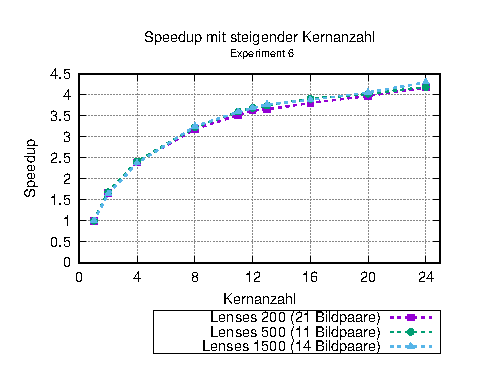
\includegraphics[width=\textwidth]{pdf/speedup_exp6}
		\caption[Experiment 6]{Experiment 6}
		\label{fig:speedup_exp6}
	\end{subfigure}
	\hfill
	\begin{subfigure}[b]{0.325\textwidth}
		\centering
		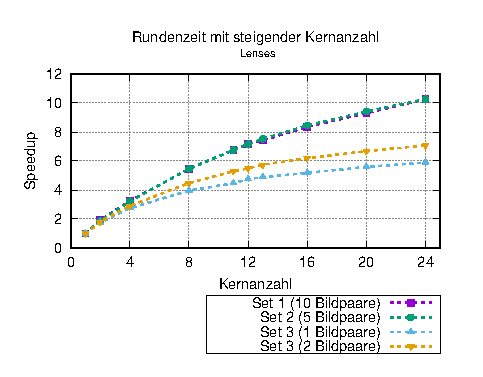
\includegraphics[width=\textwidth]{pdf/speedup_lenses}
		\caption[Lenses]{Lenses}
		\label{fig:speedup_lenses}
	\end{subfigure}
	\caption{Speedup}
\end{figure}
\end{center}

\begin{center}
	\begin{figure}[htbp]
		\begin{subfigure}[b]{0.7\textwidth}
			\centering
			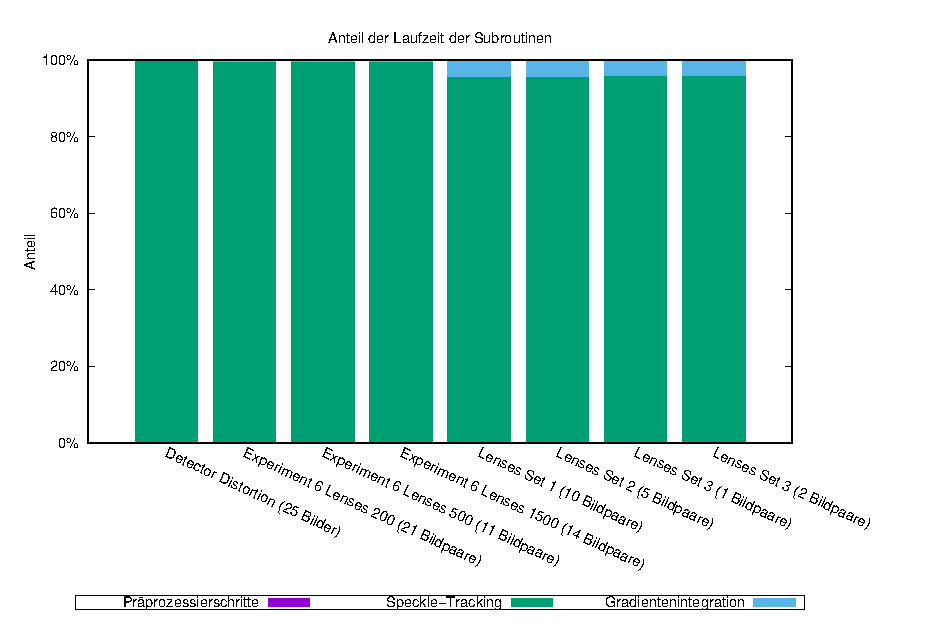
\includegraphics[width=\textwidth]{pdf/main}
			\caption{Anteile der Laufzeiten}
			\label{fig:perc_main}
		\end{subfigure}
		
		\begin{subfigure}[b]{0.7\textwidth}
			\centering
			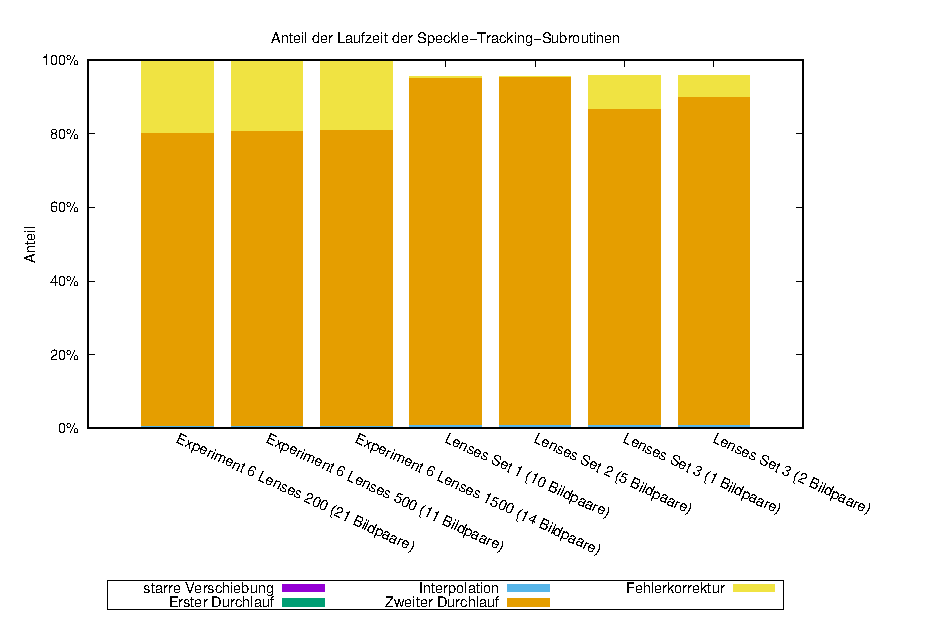
\includegraphics[width=\textwidth]{pdf/speckle}
			\caption{Anteile der Laufzeiten des Speckle-Tracking-Algorithmus}
			\label{fig:perc_speckle}
		\end{subfigure}
		
		\begin{subfigure}[b]{0.7\textwidth}
			\centering
			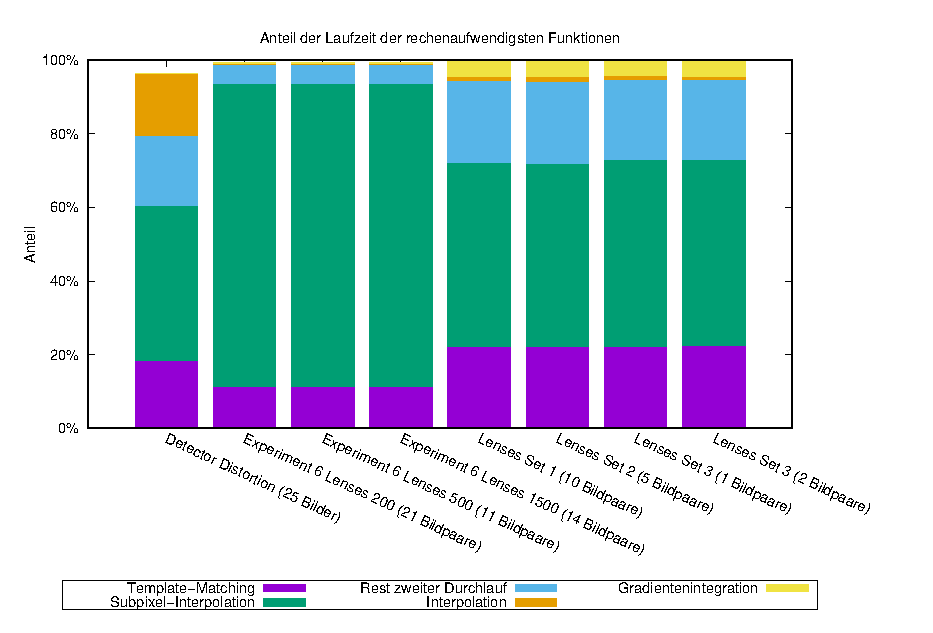
\includegraphics[width=\textwidth]{pdf/slow}
			\caption{Anteile der Laufzeiten der langsamsten Funktionen}
			\label{fig:perc_slow}
		\end{subfigure}
		\caption{Anteile der Laufzeiten}
	\end{figure}
\end{center}

\section{Grund der Performance-Engpässe}

\begin{correctmore}
	- Python
	- Overhead in der joblib
	- häufige Aufrufe von norm\_xcorr un nxcorr\_disp
	- niedrige CPU util
	- siehe tmp
\end{correctmore}